\documentclass[12pt]{article}

\usepackage[a4paper, margin=1in]{geometry}

\usepackage{listings}
\usepackage{color}
\usepackage{float}
\usepackage{graphicx}
\usepackage{subcaption}

\definecolor{codegreen}{rgb}{0,0.6,0}
\definecolor{codegray}{rgb}{0.5,0.5,0.5}
\definecolor{codepurple}{rgb}{0.58,0,0.82}
\definecolor{backcolour}{rgb}{0.95,0.95,0.92}

\lstdefinestyle{mystyle}{
  backgroundcolor=\color{backcolour},
  commentstyle=\color{codegreen},
  keywordstyle=\color{magenta},
  numberstyle=\tiny\color{codegray},
  stringstyle=\color{codepurple},
  basicstyle=\ttfamily,
  breakatwhitespace=false,
  breaklines=true,
  captionpos=b,
  keepspaces=true,
  numbers=left,
  numbersep=5pt,
  showspaces=false,
  showstringspaces=false,
  showtabs=false,
  tabsize=2
}

\lstset{style=mystyle}

\setlength\parindent{0pt}
\setlength\parskip{1em}

\title{Lab 7 - Reduction}
\author{\textsc{Nguyen} Duc Tung}
\date{}

\begin{document}

\maketitle

This lab objective is to stretch the greyscale of an image. This includes two steps:

\begin{enumerate}
  \item Find max/min intensity
  \item Recalculate the intensity for each pixel
\end{enumerate}

Step 2 can be easily done by inplement Map using a formula. But step 1 will be done by a Reduction to find the max/min. The reduction is done and optimized by following the instructions on the lecture. However, 1 block can only processed a small part of the images, we can not do 1 reduction and get the global result. Therefore, we need a blocks synchronization method call the reduction kernel again and again, until we reach only 1 output.
\\\\
My idea is to used two pointers, 1 for the input, 1 for the output. After each kernel run finished, the pointers is swapped, so that output of this run will be the input of the next run. And it will continually invoking the kernel until we get the desired max/min. Following snippet of code explains my approach:
\\
\begin{lstlisting}[language=C]
while (reduceGridSize > 1) {
    getMaxIntensity<<<reduceGridSize, blockSize, threadsPerBlock>>>(maxArrayPointer[swap], maxArrayPointer[!swap]);

    reduceGridSize = (reduceGridSize + threadsPerBlock - 1) / threadsPerBlock;
    swap = !swap;
}
\end{lstlisting}

\pagebreak

Here is an image with greyscale stretched:

Time elapsed: 29.9 ms

\begin{figure}[H]
  \centering
  \begin{subfigure}{.45\textwidth}
    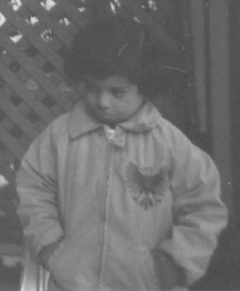
\includegraphics[width=\linewidth]{./img/in.jpg}
    \caption{Original image}
  \end{subfigure}
  \hspace{1cm}
  \begin{subfigure}{.45\textwidth}
    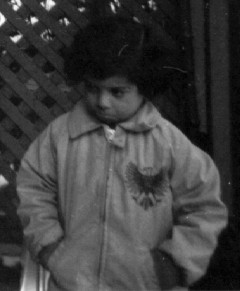
\includegraphics[width=\linewidth]{./img/out.jpg}
    \caption{Greyscale stretched}
  \end{subfigure}
\end{figure}

\end{document}
